\documentclass[paper=a4,fontsize=10pt,baselineskip=15pt]{jlreq}
\usepackage{kk}
\usepackage{graphicx,booktabs,array,titlesec}
\usepackage{hyperref}
\hypersetup{luatex,pdfencoding=auto,colorlinks=true,urlcolor=blue,pdftitle={SmolVLAの8タスク追加学習とROS 2評価},pdfauthor={},pdfcreationdate={},pdfmoddate={}}
\titleformat{\section}{\large\bfseries}{\thesection.}{.6em}{}
\titleformat{\subsection}{\normalsize\bfseries}{}{0em}{}
\titlespacing*{\section}{0pt}{9pt}{4pt}
\titlespacing*{\subsection}{0pt}{6pt}{3pt}
\setlength{\parindent}{1em}
\setlength{\parskip}{3pt}
\renewcommand{\arraystretch}{1.18}
\newcommand{\repo}{https://github.com/lemonydrink/PhysicalAI-final}
\begin{document}
\begin{center}
{\LARGE\bfseries SmolVLAの8タスク追加学習とROS 2評価}\\[5pt]
{\large LIBERO-PLUSによるSFT・性能比較・軌道の可視化}
\end{center}
\section{DATA}
Franka Pandaシミュレーションの8タスクを対象とする実験報告。モデル評価と最終ROS 2評価を分けて論じる。詳細な設定・全評価記録・失敗実験・動画・LeRobotデータは公開リポジトリ[1]に保存した。
\section{背景・目的}
PARCコンペでSmolVLAがπ0.5に匹敵する性能を発揮した参加者がいたという報告に着想を得て、\textbf{8タスクと利用可能な計算資源の範囲でSmolVLAの最高性能を目指した}。最低目標は成功率70\%と全8タスクの成功動画とした。PARCの事例は動機であり、本実験でπ0.5との直接比較は行っていない。

対象は牛乳・トマトソース・バターの収納、ボウル3種の移動、引き出し、皿押し。X-VLA／2toINFの参照系から出発したが、最終的にはSmolVLAのAction Expert中心のSFTへ移行した。
\section{本論}
\subsection{初期の失敗と学習系の修正}
\begin{center}
\begin{tabular}{@{}lr@{}}\toprule
系列・段階 & 保存された成功数 \\\midrule
公式汎用baseからの初期SFT & 1/80（1.25\%）\\
公式LIBERO-PLUSからの初期SFT & 5/80（6.25\%）\\
LIBERO-PLUS系列の全件1巡継続学習 & 3/80（3.75\%）\\
入力等の修正後・別系列LIBERO-PLUS baseline & 80/80\\
同系列の2,000更新 & 78/80\\\bottomrule
\end{tabular}
\end{center}
初期SFTは期待する結果を残せず、画像向き・姿勢表現・有効7次元loss・FP32重みとBF16演算・正規化を監査した。低成績は監査前の実装条件を含み、公式モデルの性能上限を示さない。batch4×蓄積8からbatch32×蓄積1へ変更した別系列は途中で停止し、公開BurgQモデル[2]からbaseline測定と新規optimizerによるSFTを開始した。
\subsection{データと最終学習条件}
\texttt{Sylvest/libero\_plus\_lerobot}の対象8タスク3,071 episode・404,716 frameを使用。全件で元Parquetと学習HDF5のstate/action一致を確認した。操作列hashの350グループで分割し、検証306本すべてに生じていた学習側との操作列重複を解消した。学習2,779本・365,887 frame、検証292本・38,829 frame。元LIBEROと一致する拡張軌道を含み、独立した3,071種類の操作列ではない。

BurgQ付属の正規化を維持し、front／wrist RGB＋state8Dからrelative OSC7Dを出力する。VLMを凍結しAction Expertとstate/action projection約99.88Mを学習。AdamW、batch32、蓄積1、LR最大$3\times10^{-5}$、warmup572更新、cosineで最終$3\times10^{-6}$、weight decay $10^{-4}$、clip norm1.0。学習は1 epoch・11,434更新で全学習frameを各1回使用。W\&B offlineとJSONLに記録した。
\subsection{軌道データの記録と検証}
元評価の各step状態・指令は未保存だったため、同じモデル・seed・初期状態でROS 2再実行して記録した。\textbf{再実行の正面MP4は8本すべて元採用クリップとSHA256・全973復号frameが一致}したが、元の未記録の内部状態・指令との直接一致は検証できない。
LeRobot v3.0に8 episode・973観測・965実行指令、2カメラ、関節角・速度を収録した。終端8行のactionは仮置きで\texttt{action.valid=false}。全行の主要状態・指令を生記録と照合し、24地点で両カメラの読み込みを検証した。詳細な時系列図は[1]に掲載。再圧縮したデータセット映像の元画像との画素一致は主張しない。
\newpage
\subsection{モデル性能：同じ80試行での追加学習前後比較}
各タスク10試行、最大300 step、制御周期0.05秒。baselineと各checkpointは初期状態index10〜19を用い、全80件でseed・初期状態hashの一致を確認した。以下は\textbf{HTTP経由のモデル比較・checkpoint選択用セット}であり、最終ROS 2セットとは分ける。
\begin{center}
\begin{tabular}{@{}rcrr@{}}\toprule
更新数 & 成功数 & 成功率 & 無衝突成功数 \\\midrule
0（公開モデル） & 73/80 & 91.25\% & 60/80\\
2,000 & 69/80 & 86.25\% & 53/80\\
4,000 & 77/80 & 96.25\% & 63/80\\
6,000 & 76/80 & 95.00\% & 61/80\\
8,000 & 73/80 & 91.25\% & 60/80\\
10,000 & 73/80 & 91.25\% & 62/80\\
\textbf{11,434} & \textbf{78/80} & \textbf{97.50\%} & \textbf{63/80}\\\bottomrule
\end{tabular}
\end{center}
最終checkpointを成功数優先で選択した。\textbf{成功率は+6.25ポイント}、無衝突成功率は75.00\%から78.75\%へ\textbf{+3.75ポイント}。更新数に対して単調な改善ではなかった。
\begin{center}
\begin{tabular}{@{}lccc@{}}\toprule
タスク & 学習前 & 学習後 & 無衝突成功・前→後\\\midrule
牛乳→バスケット & 8/10 & 10/10 & 8→10\\
トマトソース→バスケット & 9/10 & 10/10 & 9→10\\
バター→バスケット & 10/10 & 10/10 & 10→10\\
ボウル（中央）→皿 & 9/10 & 10/10 & 8→8\\
ボウル（クッキー側）→皿 & 8/10 & 10/10 & 6→3\\
ボウル→皿 & 10/10 & 10/10 & 10→10\\
引き出し & 9/10 & 10/10 & 9→10\\
皿押し & 10/10 & 8/10 & 0→2\\\midrule
合計 & 73/80 & 78/80 & 60→63\\\bottomrule
\end{tabular}
\end{center}
対応付きで失敗→成功7件、成功→失敗2件、成功維持71件。皿押しの成功率は低下し、クッキー側ボウルは成功数増加と同時に無衝突成功数が減った。改善の中心はタスク完了であり、無衝突性の全面的な改善ではない。

\textbf{無衝突の定義：}非対象物の最大変位が1 mmを超えた場合をcollisionとする補助指標。無衝突成功率は「成功かつcollisionなし」／全80試行であり、接触センサーで全接触の不存在を検証した意味ではない。
\subsection{Loss・モデル選択と解釈}
中間64サンプルのvalidation lossは2,000更新0.541から10,000更新0.728へ上昇したが、rollout成績の順位とは一致しなかった。最終loss0.728は検証38,829 frame全件の値で、中間値と同一母集団の比較ではない。

同じ80試行で6個のcheckpointを選んだため選択バイアスがある。+6.25ポイントはこのセットでの観測値であり、独立した汎化性能の改善を確証しない。公開baseline自体が70\%を上回り、別系列には80/80もあるため、今回の方式が全候補中で最高とは結論しない。
\newpage
\subsection{最終ROS 2評価：固定モデルと別初期状態80試行}
モデル選択後に重みを固定し、初期状態index20〜29を用い、DDS経由でシミュレーター2台を並列実行した。SmolVLA→HTTP環境間adapter→ROS 2 gateway→DDS ActionChunk→robot node→simulatorとし、観測もDDSで返す。trial別RNGとaction queueを分離した。
\begin{center}
\begin{tabular}{@{}lccc@{}}\toprule
評価区分 & 成功率 & 無衝突成功率 & 初期状態\\\midrule
モデル学習前・HTTP & 73/80（91.25\%） & 60/80（75.00\%） & 10〜19\\
選択モデル・HTTP & 78/80（97.50\%） & 63/80（78.75\%） & 10〜19\\
最終ROS 2・2並列 & 78/80（97.50\%） & 68/80（85.00\%） & 20〜29\\\bottomrule
\end{tabular}
\end{center}
最終ROS 2はインフラエラー0件、9,782 actionでDDS受信数とsimulator step数が一致した。失敗は牛乳1件、中央ボウル1件。HTTPとの無衝突成功数の差は初期状態も異なるため、ROS 2による性能向上と解釈しない。
\subsection{成果動画とLeRobot形式の軌道資料}
全8タスクの無衝突成功例を1本ずつ選び、プロンプト付きMP4と軌道資料を作成した。軌道は同条件で再実行して記録したもので、元評価の未保存ログではない。
\begin{center}
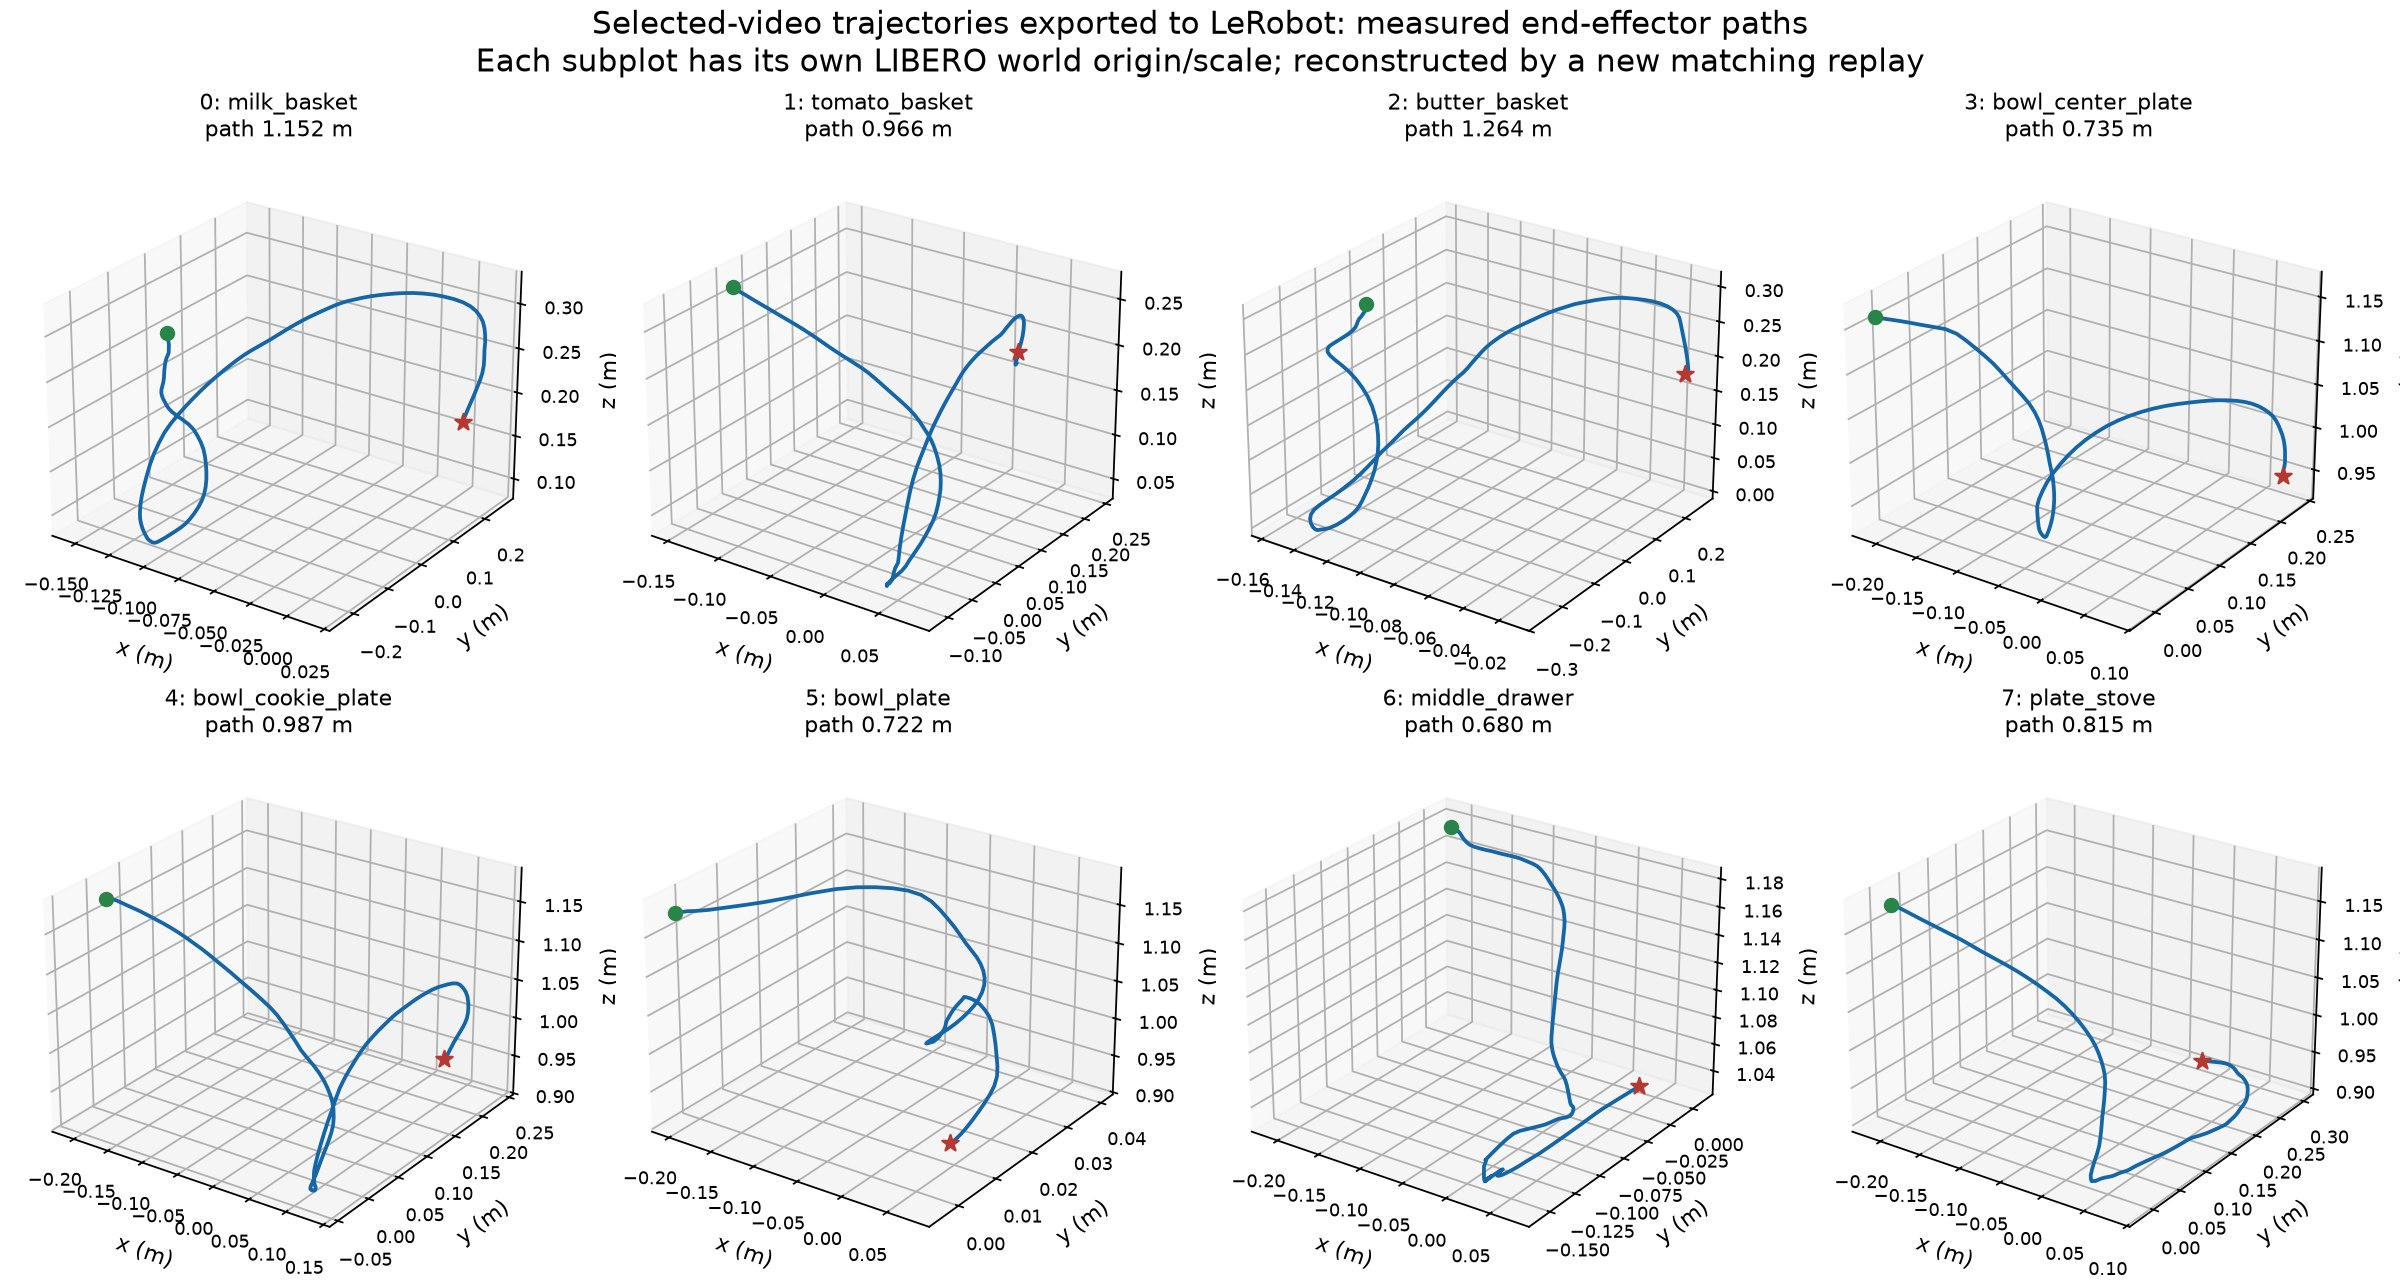
\includegraphics[width=.84\linewidth]{trajectory_overview.jpg}\\[-1pt]
{\small 図1：変換後のLeRobotデータから描画した手先軌道。緑は開始、赤は終端。\\タスクごとにworld原点・縮尺が異なる。再実行で測定した軌道である。}
\end{center}
\section{考察}
成功例8件の動画・軌道は性能推定用の無作為標本ではない。最終80試行の無衝突成功率は85\%であり、選択動画の8/8を100\%性能と扱わない。BurgQ事前学習と元LIBEROの重複、8基本タスクへの限定も残る。実機driver接続・校正・下位制御・非常停止の実機検証は未完で、実機成功は主張しない。
\section{結論}
BurgQからの1 epoch SFTで選択用セットの成功率97.5\%（+6.25ポイント）を観測し、別セットのROS 2実行でも97.5\%を得た。目標70\%と8タスクの動画・軌道資料は達成した。残る課題は無衝突性、独立条件での改善確認、実機検証である。
\section{参考文献}
{\small [1] \href{\repo/tree/main/reports/experiment-burgq/final-report}{PhysicalAI-final：詳細報告・評価記録・軌道データ}（GitHub）。\par
[2] \href{https://huggingface.co/BurgQ/smolvla-libero-bs32-100k}{BurgQ/smolvla-libero-bs32-100k}（初期モデル）。}
\end{document}
